% Options for packages loaded elsewhere
\PassOptionsToPackage{unicode}{hyperref}
\PassOptionsToPackage{hyphens}{url}
%
\documentclass[
]{article}
\usepackage{lmodern}
\usepackage{amssymb,amsmath}
\usepackage{ifxetex,ifluatex}
\ifnum 0\ifxetex 1\fi\ifluatex 1\fi=0 % if pdftex
  \usepackage[T1]{fontenc}
  \usepackage[utf8]{inputenc}
  \usepackage{textcomp} % provide euro and other symbols
\else % if luatex or xetex
  \usepackage{unicode-math}
  \defaultfontfeatures{Scale=MatchLowercase}
  \defaultfontfeatures[\rmfamily]{Ligatures=TeX,Scale=1}
\fi
% Use upquote if available, for straight quotes in verbatim environments
\IfFileExists{upquote.sty}{\usepackage{upquote}}{}
\IfFileExists{microtype.sty}{% use microtype if available
  \usepackage[]{microtype}
  \UseMicrotypeSet[protrusion]{basicmath} % disable protrusion for tt fonts
}{}
\makeatletter
\@ifundefined{KOMAClassName}{% if non-KOMA class
  \IfFileExists{parskip.sty}{%
    \usepackage{parskip}
  }{% else
    \setlength{\parindent}{0pt}
    \setlength{\parskip}{6pt plus 2pt minus 1pt}}
}{% if KOMA class
  \KOMAoptions{parskip=half}}
\makeatother
\usepackage{xcolor}
\IfFileExists{xurl.sty}{\usepackage{xurl}}{} % add URL line breaks if available
\IfFileExists{bookmark.sty}{\usepackage{bookmark}}{\usepackage{hyperref}}
\hypersetup{
  pdftitle={varameta::},
  hidelinks,
  pdfcreator={LaTeX via pandoc}}
\urlstyle{same} % disable monospaced font for URLs
\usepackage[margin=1in]{geometry}
\usepackage{graphicx}
\makeatletter
\def\maxwidth{\ifdim\Gin@nat@width>\linewidth\linewidth\else\Gin@nat@width\fi}
\def\maxheight{\ifdim\Gin@nat@height>\textheight\textheight\else\Gin@nat@height\fi}
\makeatother
% Scale images if necessary, so that they will not overflow the page
% margins by default, and it is still possible to overwrite the defaults
% using explicit options in \includegraphics[width, height, ...]{}
\setkeys{Gin}{width=\maxwidth,height=\maxheight,keepaspectratio}
% Set default figure placement to htbp
\makeatletter
\def\fps@figure{htbp}
\makeatother
\setlength{\emergencystretch}{3em} % prevent overfull lines
\providecommand{\tightlist}{%
  \setlength{\itemsep}{0pt}\setlength{\parskip}{0pt}}
\setcounter{secnumdepth}{5}
\newlength{\cslhangindent}
\setlength{\cslhangindent}{1.5em}
\newenvironment{cslreferences}%
  {\setlength{\parindent}{0pt}%
  \everypar{\setlength{\hangindent}{\cslhangindent}}\ignorespaces}%
  {\par}

\title{varameta::}
\author{}
\date{\vspace{-2.5em}}

\begin{document}
\maketitle

{
\setcounter{tocdepth}{2}
\tableofcontents
}
\begin{verbatim}
# for reproducibility
set.seed(39)

# packages
library(varameta)
library(tidyverse)
library(simeta)
library(panda)

# move to parameter when done with chunk-wise?
sample_size <- 10
\end{verbatim}

\hypertarget{objective-of-the-varameta-package}{%
\section{\texorpdfstring{Objective of the \texttt{varameta::}
package}{Objective of the varameta:: package}}\label{objective-of-the-varameta-package}}

The \texttt{varameta::} package aims to bridge the toolchain gap from a
dataset containing medians to a software package, such as
\texttt{metafor::} (Viechtbauer 2010), for meta-analysis.

\begin{verbatim}
panda("varameta:: is for meta-analysing medians")
#> Set panda = 41 to reproduce this panda.
\end{verbatim}

\begin{center}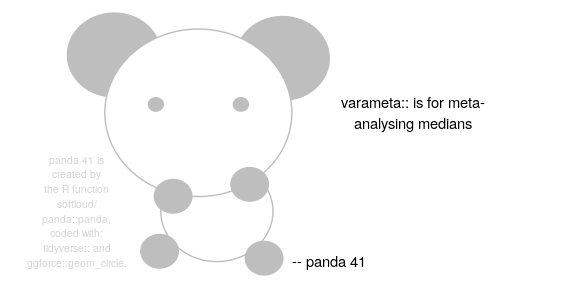
\includegraphics{varameta_files/figure-latex/unnamed-chunk-2-1} \end{center}

\hypertarget{a-minimal-demonstration-of-calculating-the-variance-of-the-sample-median}{%
\section{A minimal demonstration of calculating the variance of the
sample
median}\label{a-minimal-demonstration-of-calculating-the-variance-of-the-sample-median}}

\begin{verbatim}
panda("show me the code!")
#> Set panda = 30 to reproduce this panda.
\end{verbatim}

\begin{center}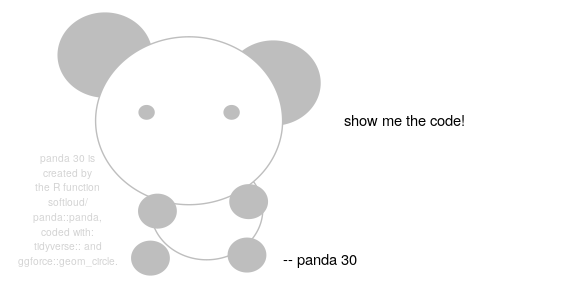
\includegraphics{varameta_files/figure-latex/unnamed-chunk-3-1} \end{center}

\hypertarget{compute-standard-error-of-the-sample-median}{%
\subsection{Compute standard error of the sample
median}\label{compute-standard-error-of-the-sample-median}}

\begin{verbatim}
# get a sample
a_sample <- rexp(sample_size)

# get standard error of the sample median
effect_se(
  centre = median(a_sample),
  spread = IQR(a_sample),
  n = length(a_sample),
  centre_type = "median",
  spread_type = "iqr"
)
#> [1] 0.1400956
\end{verbatim}

\hypertarget{vectorised-calculations-for-dataframes}{%
\subsection{Vectorised calculations for
dataframes}\label{vectorised-calculations-for-dataframes}}

Here we borrow a function from the companion \texttt{simeta::} package.
See below for details.

\begin{verbatim}
# generate random meta-analysis dataset
# one row per study
(ma_sample <- sim_stats() %>%
  # filter down to one group per study
  dplyr::filter(group == "control"))
#> # A tibble: 3 x 5
#>   study   group   effect effect_spread     n
#>   <chr>   <chr>    <dbl>         <dbl> <dbl>
#> 1 study_1 control   48.4         0.310    93
#> 2 study_2 control   47.3         0.350    36
#> 3 study_3 control   59.2         0.275    65


ma_sample %>%
  # append a column with the standard error of the median for each study
  mutate(effect_se = pmap_dbl(
    list(centre = effect,
         spread = effect_spread,
         n = n),
    effect_se,
    centre_type = "median",
    spread_type = "iqr"
  ))
#> # A tibble: 3 x 6
#>   study   group   effect effect_spread     n effect_se
#>   <chr>   <chr>    <dbl>         <dbl> <dbl>     <dbl>
#> 1 study_1 control   48.4         0.310    93    0.0298
#> 2 study_2 control   47.3         0.350    36    0.0542
#> 3 study_3 control   59.2         0.275    65    0.0317
\end{verbatim}

\hypertarget{calculate-the-standard-error-of-mean-or-median-based-on-effect-spread-and-sample-size}{%
\section{Calculate the standard error of mean or median based on effect,
spread, and sample
size}\label{calculate-the-standard-error-of-mean-or-median-based-on-effect-spread-and-sample-size}}

A wrapper function \texttt{effect\_se} provides a quick method of
calculating the error of an effect based on its measure of effect,
spread, sample size.

Consider a randomly generated sample.

\begin{verbatim}
(a_sample <- rlnorm(sample_size,-1, 0.1))
#>  [1] 0.3534391 0.3395523 0.3876237 0.2869194 0.3688613 0.3874923 0.4324285 0.4337460 0.3388299 0.3449407

# summary statistics for this sample
a_sample %>% log() %>% summary()
#>    Min. 1st Qu.  Median    Mean 3rd Qu.    Max. 
#> -1.2486 -1.0762 -1.0187 -1.0082 -0.9478 -0.8353
\end{verbatim}

Taken from a lognormal distribution \(\mathrm{lognormal}(-1, 0.1^2)\).

\begin{center}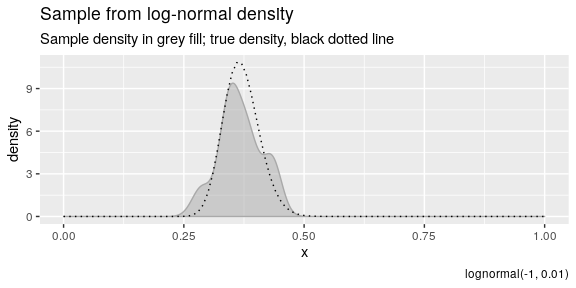
\includegraphics{varameta_files/figure-latex/plot-1} \end{center}

\hypertarget{estimate-the-standard-error-of-the-sample-median}{%
\subsection{Estimate the standard error of the sample
median}\label{estimate-the-standard-error-of-the-sample-median}}

With the \texttt{varameta::} package we execute the following code to
estimate the standard error of the sample median, with sample summary
statistics: \texttt{median}; \texttt{IQR} (interquartile range);
\texttt{length} for sample size.

\begin{verbatim}
# standard error based on the median, interquartile range, and sample size
effect_se(
  centre = median(a_sample),
  spread = IQR(a_sample),
  n = length(a_sample),
  centre_type = "median",
  spread_type = "iqr"
)
#> [1] 0.01370849
\end{verbatim}

The calculation can be adapted for the range.

\begin{verbatim}
# standard error based on the median, range, and sample size
effect_se(
  centre = median(a_sample),
  spread = abs(diff(range(a_sample))),
  n = length(a_sample),
  centre_type = "median",
  spread_type = "range"
)
#> [1] 0.01756955
\end{verbatim}

\begin{verbatim}
panda("show me the math!")
#> Set panda = 12 to reproduce this panda.
\end{verbatim}

\begin{center}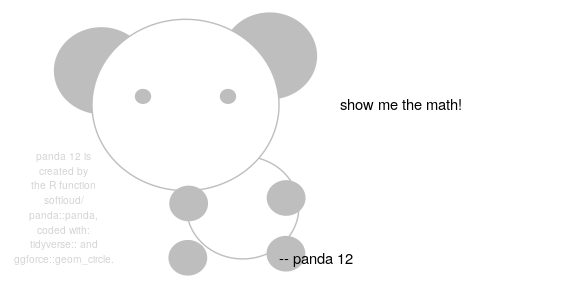
\includegraphics{varameta_files/figure-latex/unnamed-chunk-6-1} \end{center}

This calculation

todo: eqn to finish off section! words around eqns to finish off section
blah blah see companion manuscript..

\[
\mathrm v(M) := \frac 1 {4n\left[ g\left(M; \hat{\theta}\right)\right]^2}
\]

\[
\hat \mu := \log(M).
\]

\[
G^{-1}(p; \mu, \sigma) = \exp(\sigma\Phi^{-1}(p) + \mu).
\]

\[
\hat{\sigma}^{(1)} := \frac 1 {\Phi^{-1}\left(\frac 3 4\right)} \log\left(\frac {\mathrm{iqr} e^{- \hat \mu} \pm
\sqrt{\mathrm{iqr}^2 e^{-2 \hat \mu} + 4}
} {2}\right)
\]

\[
\hat{\sigma}^{(2)} := \frac 1 {\Phi^{-1}\left(\frac {n - \frac 1 2} n\right)} \log\left[\frac {(x_{[n]} - x_{[1]}) e^{- \hat \mu} \pm
\sqrt{(x_{[n]} - x_{[1]})^2 e^{-2\hat \mu} + 4}
} {2}\right].
\]

\hypertarget{calculate-the-standard-error-of-the-sample-mean}{%
\subsection{Calculate the standard error of the sample
mean}\label{calculate-the-standard-error-of-the-sample-mean}}

\begin{verbatim}
# take a sample
se_mean_eg_sample <- rexp(sample_size)
\end{verbatim}

Now, we wish to calculate the standard error \(s/\sqrt n\) of the sample
mean, calcualted with the the sample standard deviation and the
squared-root of the sample size.

\begin{verbatim}
# mean and sd
effect_se(
  centre = mean(se_mean_eg_sample),
  spread = sd(se_mean_eg_sample),
  n = length(se_mean_eg_sample),
  centre_type = "mean",
  spread_type = "sd"
)
#> [1] 0.1548837

# compare
sd(se_mean_eg_sample) /
  sqrt(length(se_mean_eg_sample))
#> [1] 0.1548837

# mean and var
effect_se(
  centre = mean(se_mean_eg_sample),
  spread = var(se_mean_eg_sample),
  n = length(se_mean_eg_sample),
  centre_type = "mean",
  spread_type = "var"
)
#> [1] 0.1548837

# compare
sqrt(var(se_mean_eg_sample) /
  length(se_mean_eg_sample))
#> [1] 0.1548837
\end{verbatim}

\hypertarget{vectorised-calculations-for-meta-analysis-datasets}{%
\section{Vectorised calculations for meta-analysis
datasets}\label{vectorised-calculations-for-meta-analysis-datasets}}

\begin{verbatim}
panda("vectorisation is my favourite part of R", panda = 14)
#> Set panda = 14 to reproduce this panda.
\end{verbatim}

\begin{center}\includegraphics{varameta_files/figure-latex/unnamed-chunk-9-1} \end{center}

\begin{verbatim}
# borrowing from sister package simeta:: to simulate a dataset
(meta_data <- sim_stats() %>% 
  dplyr::filter(group == "control"))
#> # A tibble: 3 x 5
#>   study   group   effect effect_spread     n
#>   <chr>   <chr>    <dbl>         <dbl> <dbl>
#> 1 study_1 control   64.4         0.189    19
#> 2 study_2 control   52.0         0.273    99
#> 3 study_3 control   48.6         0.190    27

# add a vecorised
# todo function this (after report)
meta_data %>% 
  mutate(
    effect_se = pmap_dbl(
      list(centre = effect, spread = effect_spread, n = n),
      effect_se,
      centre_type = "median",
      spread_type = "iqr"
    )
  )
#> # A tibble: 3 x 6
#>   study   group   effect effect_spread     n effect_se
#>   <chr>   <chr>    <dbl>         <dbl> <dbl>     <dbl>
#> 1 study_1 control   64.4         0.189    19    0.0403
#> 2 study_2 control   52.0         0.273    99    0.0255
#> 3 study_3 control   48.6         0.190    27    0.0339
\end{verbatim}

\hypertarget{other-estimators}{%
\section{Other estimators}\label{other-estimators}}

\begin{verbatim}
panda(
  panda = 49,
  "varameta:: provides several estimators for the variances of the sample median")
#> Set panda = 49 to reproduce this panda.
\end{verbatim}

\begin{center}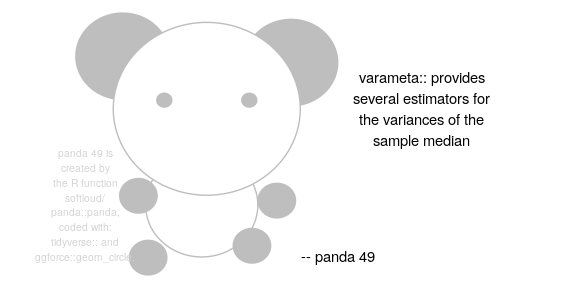
\includegraphics{varameta_files/figure-latex/unnamed-chunk-11-1} \end{center}

All other estimators available for meta-analysis are provided in
\texttt{varameta::} for use in a compative analysis.

\hypertarget{references}{%
\section*{References}\label{references}}
\addcontentsline{toc}{section}{References}

\hypertarget{refs}{}
\begin{cslreferences}
\leavevmode\hypertarget{ref-viechtbauerConductingMetaanalysesMetafor2010}{}%
Viechtbauer, Wolfgang. 2010. ``Conducting Meta-Analyses in R with the
metafor Package.'' \emph{Journal of Statistical Software} 36 (3): 1--48.
\end{cslreferences}

\end{document}
